\documentclass[aspectratio=169]{beamer}
\usepackage[utf8]{inputenc}
\usepackage{booktabs}
\usepackage{tikz}
\usetikzlibrary{positioning,arrows.meta}

\usetheme{Madrid}
\usecolortheme{default}
\definecolor{ATCBlue}{RGB}{13,53,85}
\definecolor{ATCAccent}{RGB}{22,112,173}
\setbeamercolor{structure}{fg=ATCBlue}
\setbeamercolor{palette primary}{bg=ATCBlue,fg=white}
\setbeamercolor{palette secondary}{bg=ATCAccent,fg=white}
\setbeamercolor{frametitle}{bg=ATCBlue,fg=white}
\setbeamercolor{title}{fg=ATCBlue}
\setbeamercolor{block title}{bg=ATCBlue,fg=white}
\setbeamercolor{block body}{bg=blue!4!white,fg=black}
\setbeamertemplate{navigation symbols}{}
\setbeamertemplate{footline}[frame number]
\setbeamertemplate{items}[circle]

\title[ATC Crowd Safety Explorer]{ATC Crowd Safety Explorer}
\subtitle{Trajectory History and Agent Based Crowd Simulation for Event Safety}
\author[Group 4]{\textbf{Project Team}\\
Nivin P Louis (TL23BTAI0042) \quad Niranjana Sreevalsan (TL23BTAI0348)\\
Farhan Mohamed T P (TL23BTAI0308) \quad Nihal P Shakeer (TL23BTAI0249)\\[0.35cm]
\textbf{Project Guide}\\
Anju K P, Assistant Professor, Department of AIML}
\institute[Dept. AIML]{Vidya Academy of Science and Technology, Thrissur}
\date{Project Presentation}

\begin{document}

\begin{frame}
  \titlepage
\end{frame}

\begin{frame}{Institution and department context}
\begin{columns}[T]
\begin{column}{0.18\textwidth}
\centering

\includegraphics[width=0.9\linewidth]{college_logo.png}
\end{column}
\begin{column}{0.78\textwidth}
\small
\textbf{College vision}\par
To nurture innovative engineering professionals who contribute to sustainable societal development.\vspace{0.25cm}

\textbf{Department vision}\par
To build competence in artificial intelligence and machine learning through education, research, and responsible innovation.\vspace{0.25cm}

\textbf{Project alignment}\par
This project applies data-driven modelling to public-space safety, with transparent validation and clearly stated limits.
\end{column}
\end{columns}
\end{frame}

\begin{frame}{Presentation roadmap}
\tableofcontents
\end{frame}

\section{Problem and scope}
\begin{frame}{Crowd safety problem}
\begin{block}{Operational need}
Event operators need a way to inspect current crowd conditions and test how congestion may evolve when attendance, movement patterns, or routes change.
\end{block}
\begin{itemize}
  \item Static head counts cannot describe local concentration or counter-flow.
  \item A future crowd state depends on individual paths, destinations, and local interactions.
  \item Real emergency experiments are unsafe, so scenario simulation must support planning.
\end{itemize}
\vspace{0.2cm}
\alert{Scope of this prototype:} normal-flow forecasting from recorded ATC trajectories plus controlled capacity scenarios. It does not claim to predict a real stampede.
\end{frame}

\begin{frame}{Project objectives}
\begin{enumerate}
  \item Load a selected ATC date and time, then replay observed pedestrian movement.
  \item Build multi-day behavioural profiles from trajectory data.
  \item Initialize a Social Force agent model from observed crowd positions or synthetic route zones.
  \item Infer near-term route intent from recent trajectory history.
  \item Validate short-term forecasts against later positions in a held-out ATC day.
  \item Support capacity experiments with larger synthetic crowds and route scenarios.
\end{enumerate}
\end{frame}

\section{Data and system}
\begin{frame}{ATC pedestrian tracking dataset}
\begin{columns}[T]
\begin{column}{0.53\textwidth}
\small
\begin{itemize}
  \item ATC shopping center, Osaka, Japan.
  \item Multiple 3D range sensors cover approximately 900 m\textsuperscript{2}.
  \item Ten daily CSV files currently processed in this project.
  \item Each row records time, persistent person ID, 3D position, speed, motion angle, and facing angle.
  \item A ROS occupancy grid aligns the floor plan with the tracking coordinates.
\end{itemize}
\end{column}
\begin{column}{0.43\textwidth}
\centering
\includegraphics[width=\linewidth]{../generated/atc_occupancy_map_light.png}\\[-0.05cm]
\scriptsize ATC occupancy map used for navigation constraints
\end{column}
\end{columns}
\end{frame}

\begin{frame}{Implemented system architecture}
\centering
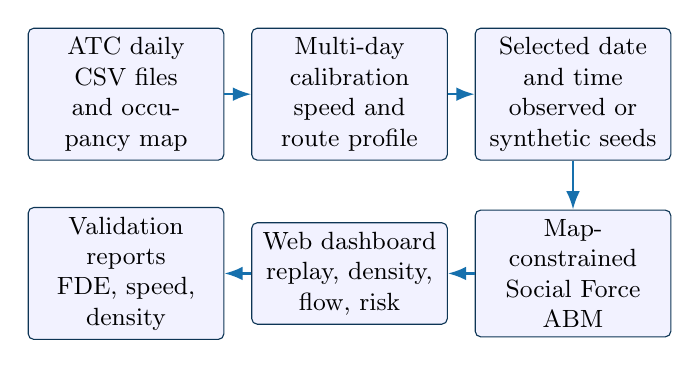
\begin{tikzpicture}[node distance=0.62cm and 0.34cm, every node/.style={font=\small,align=center}, box/.style={draw=ATCBlue,rounded corners=2pt,fill=blue!5,minimum height=1.15cm,text width=2.25cm}, arrow/.style={-Latex,thick,draw=ATCAccent}]
\node[box] (csv) {ATC daily CSV files\\and occupancy map};
\node[box,right=of csv] (profile) {Multi-day calibration\\speed and route profile};
\node[box,right=of profile] (seed) {Selected date and time\\observed or synthetic seeds};
\node[box,below=of seed] (sim) {Map-constrained\\Social Force ABM};
\node[box,left=of sim] (dashboard) {Web dashboard\\replay, density, flow, risk};
\node[box,left=of dashboard] (validation) {Validation reports\\FDE, speed, density};
\draw[arrow] (csv) -- (profile);
\draw[arrow] (profile) -- (seed);
\draw[arrow] (seed) -- (sim);
\draw[arrow] (sim) -- (dashboard);
\draw[arrow] (dashboard) -- (validation);
\end{tikzpicture}
\vspace{0.35cm}
\small The Flask dashboard runs locally and serves day selection, observed replay, simulation, and capacity-test controls.
\end{frame}

\begin{frame}{Dashboard workflow}
\begin{enumerate}
  \item Select an available tracking day and a start time in Japan Standard Time.
  \item Use \textbf{Observed replay} to inspect the recorded crowd state, density cells, speed, and flow direction.
  \item Use \textbf{Social Force ABM} with an observed snapshot for a short forecast.
  \item Select \textbf{Synthetic zone spawn} and a larger agent count for capacity scenarios.
  \item Compare normal flow, entrance surge, counter-flow, and restricted-exit conditions.
\end{enumerate}
\begin{block}{Map constraint}
Agents move only through the empirically walkable ATC footprint. This prevents simulations from crossing walls or entering untracked map regions.
\end{block}
\end{frame}

\section{Agent based model}
\begin{frame}{Agent initialization and route intent}
\begin{columns}[T]
\begin{column}{0.49\textwidth}
\begin{block}{Observed snapshot mode}
Each agent receives the tracked person ID, current position, speed, movement direction, and facing angle at the selected time.
\end{block}
\begin{block}{Trajectory history}
The system fits a velocity estimate from the previous five seconds of each person's recorded path. It uses only observations before the simulation start time.
\end{block}
\end{column}
\begin{column}{0.49\textwidth}
\begin{block}{Route intent inference}
Candidate destinations come from routes learned on other ATC days. The model weights each route using:
\begin{itemize}
\item alignment between the smoothed heading and destination;
\item compatibility between recent path origin and learned route origin;
\item observed route frequency.
\end{itemize}
\end{block}
\end{column}
\end{columns}
\end{frame}

\begin{frame}{Social Force movement model}
\small
For each agent, desired motion points along a shortest walkable path to the inferred destination. The simulator updates velocity with a relaxation term and local avoidance force.
\[
\mathbf{F}_i = \frac{v_i^0\mathbf{e}_i-\mathbf{v}_i}{\tau} + \sum_{j\ne i}\mathbf{F}_{ij}
\]
\begin{itemize}
  \item $v_i^0\mathbf{e}_i$: desired speed and direction toward the route destination.
  \item $\tau$: relaxation time that controls how quickly an agent adjusts velocity.
  \item $\mathbf{F}_{ij}$: distance-based avoidance with optional facing-angle weighting.
  \item Occupancy-map checks reject motion that would cross a wall or leave the walkable footprint.
\end{itemize}
\begin{block}{Normal-flow calibration}
The development split selected a 10.0 s relaxation time and near-zero repulsion. The low-density ATC normal-flow data did not benefit from stronger interaction forces. Dense counterfactual scenarios activate a modest avoidance force.
\end{block}
\end{frame}

\section{Validation}
\begin{frame}{Validation protocol}
\begin{columns}[T]
\begin{column}{0.53\textwidth}
\begin{enumerate}
  \item Select parameters on 11 November 2012, using three 10-second development snapshots.
  \item Exclude the current evaluation day from its multi-day speed and route profile.
  \item Hold out 14 November 2012 for final scoring.
  \item Start from six observed snapshots distributed through the held-out day.
  \item Match predicted and recorded locations using persistent person IDs at 1, 5, and 10 seconds.
\end{enumerate}
\end{column}
\begin{column}{0.43\textwidth}
\begin{block}{Metrics}
\textbf{FDE}: final displacement error in metres.\\[0.15cm]
\textbf{Speed MAE}: absolute speed error in m/s.\\[0.15cm]
\textbf{Density L1}: difference in people counts across 2 m spatial cells, normalized by observed people.
\end{block}
\end{column}
\end{columns}
\end{frame}

\begin{frame}{Held-out forecast results}
\small
\centering
\renewcommand{\arraystretch}{1.25}
\begin{tabular}{lrrrr}
\toprule
\textbf{Horizon} & \textbf{No-history FDE} & \textbf{History FDE} & \textbf{Constant velocity} & \textbf{Gain vs baseline}\\
\midrule
1 second & 0.448 m & 0.377 m & 0.458 m & 17.74\%\\
5 seconds & 2.024 m & 1.567 m & 2.338 m & 33.00\%\\
10 seconds & 4.749 m & 3.505 m & 4.986 m & 29.71\%\\
\bottomrule
\end{tabular}
\vspace{0.45cm}
\begin{block}{Result}
Five seconds of causal trajectory history improves final-position accuracy at every tested horizon. At 10 seconds, the model reduces mean error from 4.986 m for the constant-velocity baseline to 3.505 m.
\end{block}
\end{frame}

\begin{frame}{Density validation results}
\small
\centering
\renewcommand{\arraystretch}{1.35}
\begin{tabular}{lrrr}
\toprule
\textbf{Horizon} & \textbf{History density L1} & \textbf{Baseline density L1} & \textbf{Error reduction}\\
\midrule
1 second & 0.473 & 0.529 & 10.59\%\\
5 seconds & 1.032 & 1.441 & 28.38\%\\
10 seconds & 1.364 & 1.805 & 24.43\%\\
\bottomrule
\end{tabular}
\vspace{0.4cm}
\begin{itemize}
\item The model improves the spatial distribution of people, not only individual endpoints.
\item The largest density improvement occurs at the five-second horizon.
\item These scores measure ordinary ATC movement and provide the baseline for safety scenario analysis.
\end{itemize}
\end{frame}

\section{Capacity scenarios}
\begin{frame}{Capacity-test scenarios}
\begin{columns}[T]
\begin{column}{0.48\textwidth}
\begin{block}{User-configurable inputs}
\begin{itemize}
\item synthetic agent count from 20 to 1,000;
\item simulation duration from 1 to 10 minutes;
\item scenario type and selected ATC day;
\item normal, surge, counter-flow, or restricted-exit movement.
\end{itemize}
\end{block}
\end{column}
\begin{column}{0.48\textwidth}
\begin{block}{Outputs for comparison}
\begin{itemize}
\item people in view and mean speed;
\item peak local density in people/m\textsuperscript{2};
\item slow dense cells and mixed-flow cells;
\item destination arrivals and replayable trajectories.
\end{itemize}
\end{block}
\end{column}
\end{columns}
\vspace{0.22cm}
\alert{Use case:} increment agent count under the same scenario and observe when congestion indicators or flow degradation become unacceptable.
\end{frame}

\begin{frame}{Interpreting the safety claim}
\begin{block}{What the current validation supports}
The system forecasts ordinary pedestrian movement better than a constant-velocity baseline and can reproduce near-future crowd concentration more accurately on a held-out day.
\end{block}
\begin{alertblock}{What it does not yet establish}
The ATC data contain normal shopping-center movement, not labeled stampede or crowd-crush events. The project therefore provides decision support and counterfactual capacity testing, not a certified stampede-prediction system.
\end{alertblock}
\begin{itemize}
\item Capacity thresholds require domain-expert approval.
\item Real deployments require camera calibration, privacy controls, and live tracking reliability checks.
\item Emergency validation needs additional evacuation or incident data.
\end{itemize}
\end{frame}

\section{Future work}
\begin{frame}{Next development steps}
\begin{enumerate}
\item Repeat held-out validation over more dates and report confidence intervals.
\item Add scenario reports for hotspot duration, exit throughput, conflict rate, and time above a density threshold.
\item Validate route zones against the ATC entry and exit floor plan.
\item Connect a computer-vision tracking module that converts camera detections into the same floor-plan coordinate system.
\item Define operational alert rules with event-safety experts.
\end{enumerate}
\end{frame}

\section{Conclusion}
\begin{frame}{Conclusion}
\begin{itemize}
\item The project combines real ATC trajectories, map constraints, multi-day behaviour profiles, and Social Force simulation in a working dashboard.
\item A five-second trajectory-history and route-intent module improves held-out 10-second FDE by 29.71\% against constant velocity.
\item The dashboard supports replay, short-term forecasting, and synthetic crowd capacity scenarios.
\item The next evaluation stage focuses on safety indicators and expert-defined capacity thresholds.
\end{itemize}
\vfill
\centering
\Large\color{ATCBlue}\textbf{Thank you}
\end{frame}

\begin{frame}{References}
\footnotesize
\begin{enumerate}
\item ATR Digital Human Research Center. \textit{ATC pedestrian tracking dataset}, Osaka, Japan. \url{https://dil.atr.jp/crest2010_HRI/ATC_dataset/}
\item D. Helbing and P. Moln\'ar. Social force model for pedestrian dynamics. \textit{Physical Review E}, 1995.
\item F. Makinoshima and Y. Oishi. Crowd flow forecasting via agent-based simulations with sequential latent parameter estimation from aggregate observation. \textit{Scientific Reports}, 2022.
\item S. Khan and Z. Deng. Agent-based crowd simulation: an in-depth survey of determining factors for heterogeneous behaviour. \textit{The Visual Computer}, 2024.
\end{enumerate}
\end{frame}

\end{document}
